
%%%%%%%%%%%%%%%%%%%%%%%%%%%%%%%%%%%%%%%%%%%%%%%%%%
%%                                              %%
%%            Início da Introdução              %%
%%                                              %%
%%%%%%%%%%%%%%%%%%%%%%%%%%%%%%%%%%%%%%%%%%%%%%%%%%

\newpage

\chapter{Introdução}
\label{cha:intro}

\markright{}

\section{Contextualização e Problema}
\label{sec:context-problema}

A mineração de dados, ou \textit{data mining}, é um conjunto de métodos e técnicas de vital importância na análise de dados, bem como no processo de tomada de decisão, tendo sido adotada por diversas entidades para os mais diversificados objetivos. Tais entidades, normalmente empresas ou instituições,  buscam compreender melhor seus clientes, parceiros comerciais e demais colaboradores através da descoberta de padrões de comportamento existente nos dados analisados.

Mineração de dados trata, portanto, da solução de problemas através da análise do conteúdo em  bases de dados. \citeonline{witten2011data} definem \textit{data mining} como um processo automático ou semiautomático de descoberta de padrões em dados. Estes padrões devem ser significativos, ou seja, devem trazer vantagens ao usuário e os dados devem estar presentes em quantidade substancial durante o processo. Segundo \citeonline{quilici2015sistemas}, \textit{data mining} refere-se à extração de padrões de dados, no formato de regras ou estruturas equivalentes, para a obtenção de conhecimento, como mostrado na Figura \ref{fig:data-mining}.

\begin{figure}[H]
    \centering
    \caption{Mineração de dados: busca por conhecimento nos dados}
    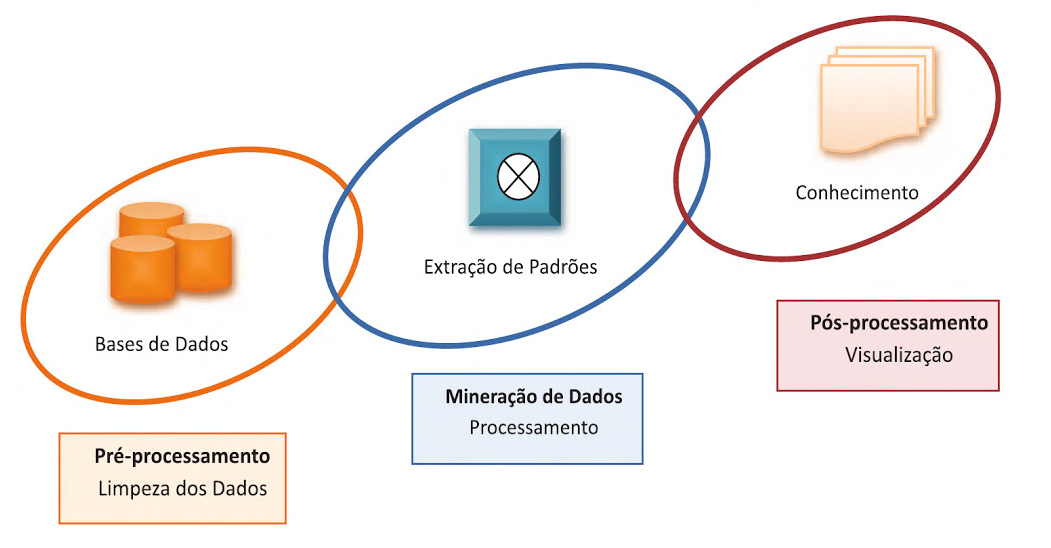
\includegraphics[width=0.8\linewidth]{figuras/data-mining.PNG}
    \source{\cite{quilici2015sistemas}.}
    \label{fig:data-mining}
\end{figure}

Um exemplo bem conhecido do uso de mineração de dados é a observação das ações de um consumidor em um mercado altamente competitivo. Através da análise do perfil e das escolhas dos clientes, pode ser possível descobrir padrões em seu comportamento, por exemplo, a quantidade de vendas em um determinado período de tempo, em relação à um período anterior. Esta análise permite identificar aqueles clientes que podem permanecer leais e os que provavelmente trocariam de marca.

Com as bases de dados ao redor do mundo em crescimento exponencial, podendo contendo dados dos mais diversos campos, há uma grande quantidade de aplicações para a mineração de dados. \citeonline{bramer2007principles} lista algumas destas aplicações, dentre elas estão: i) a detecção de fraude em cartões de crédito; ii) previsões financeira e climática; iii) diagnósticos médicos, iv) marketing direcionado ao consumidor individual; v) análise de perigo tóxico; e vi) design de produtos.

A mineração possui diferentes tarefas, que podem ser usadas para atingir objetivos diversos. \citeonline{fayyad1996kdd}, \citeonline{han2000data} e \citeonline{adhikari2014advances} mostram algumas destas tarefas, dentre as quais encontram-se: 

\begin{enumerate}[label=\roman*.]
    \item Classificação {--} Um novo dado é mapeado, ou classificado, como a uma, dentre várias classes pré\hyp{}definidas;
    \item Análise de agrupamento (\textit{clustering}) {--} Os dados são divididos em agrupamentos, mutuamente excludentes, que são determinados considerando as similaridades entre os atributos de cada item do conjunto;
    \item Sumarização {--} Provê uma descrição sumarizada (resumida) de um conjunto de dados;
    \item Regressão {--} Um dado é mapeado em um valor real, que pode ser previsto;
    \item Detecção de anomalias (\textit{outliers}) {--} Os objetos que apresentam disparidade dos outros dados analisados são detectados através da aplicação de técnicas como o cálculo da similaridade entre os objetos, observação de diferenças entre atributos ou testes estatísticos utilizando um modelo probabilístico dos dados;
    \item Regras de associação {--} Representam implicações entre os atributos de itens na base de dados, sendo que tais implicações devem corresponder a níveis de suporte e confiança fornecidos pelo usuário ao algoritmo.
\end{enumerate}

A classificação é uma tarefa que pode ser observada diariamente. De acordo com \citeonline{bramer2007principles}, classificação envolve a divisão de objetos, onde cada indivíduo é atribuído a uma dentre um número reduzido de classes pré\hyp{}definidas, sendo que cada objeto deve pertencer a uma única classe e nunca a nenhuma delas. Portanto, a classificação é o ato de atribuir rótulos, ou classes, predefinidos para objetos em uma base de dados de acordo com a semelhança entre eles.

Existem várias tarefas diárias onde o uso de classificação pode ser observado, como por exemplo: i) identificar a que os objetos mostrados em um radar correspondem (veículos, pessoas ou construções); ii) determinar a possibilidade de uma pessoa contrair uma doença (alto, médio ou baixo risco); iii) avaliar o mérito correspondente a projetos acadêmicos (ser ou não aprovado); ou iv) prever alterações de valor no mercado imobiliário (aumento ou queda de preço). A partir destes exemplos, observa-se que a tarefa de classificação está presente em diversas áreas, como saúde, marketing, mercado imobiliário ou mesmo na área militar.
	
Desta forma, para que os resultados sejam confiáveis, os dados fornecidos aos algoritmos de \textit{data mining} também devem ser. Em um mundo ideal, onde todos os sistemas interagem em harmonia e erros humanos ou computacionais não existem, as bases de dados seriam regulares, sem a presença de erros. Isto, é claro, não é o caso. Segundo \citeonline{han2000data}, as bases atuais são altamente suscetíveis a dados ruidosos, faltosos ou inconsistentes, devido tipicamente a suas dimensões (geralmente gigabytes ou mais) e possivelmente a origem dos dados (múltiplas fontes). Deste ponto em diante, neste trabalho, o termo anomalia fará referência tanto a dados faltosos, quanto a dados contendo ruídos ou inconsistências.

Para lidar com estas anomalias, existem algumas técnicas de pré\hyp{}processamento que têm por objetivo a limpeza de dados através da suavização de ruídos e correção de inconsistências. Ao trabalhar os dados antes de aplicar algum algoritmo de mineração, é possível melhorar sua eficiência e eficácia obtendo resultados mais precisos.

\begin{figure}[H]
    \centering
    \caption{Visão geral dos passos do processo de KDD}
    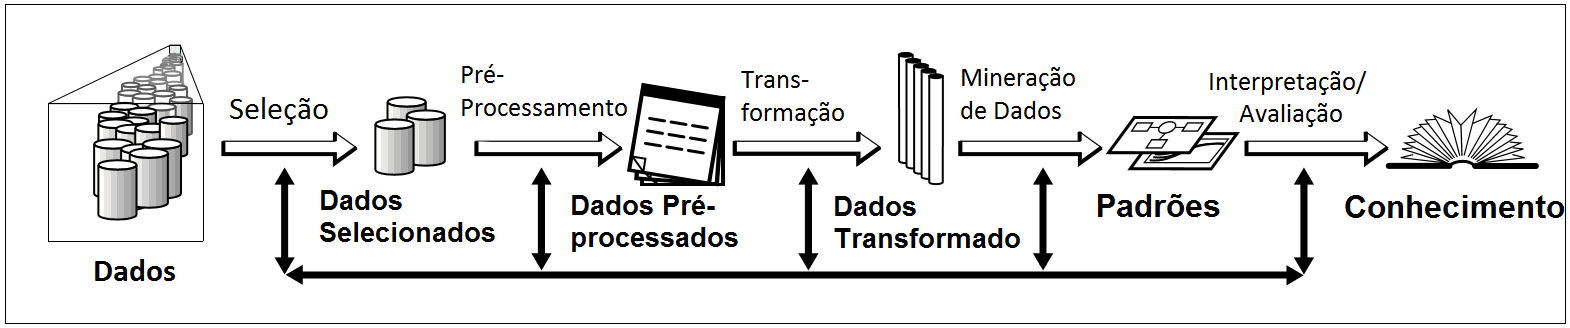
\includegraphics[width=\linewidth]{figuras/kdd-process.png}
    \source{Adaptado de \cite{fayyad1996kdd}.}
    \label{fig:kdd-process}
\end{figure}

Segundo \citeonline{fayyad1996kdd}, ambas as etapas de pré\hyp{}processamento e mineração fazem parte de um processo maior, o processo de descoberta de conhecimento em bases de dados, ou KDD (\textit{Knowledge Discovery in Databases}), que é o processo de extração de informação nova, válida, não trivial, compreensível e potencialmente útil em bases de dados. Os autores descrevem os passos do processo de KDD, envolvendo várias etapas que podem ser observadas na Figura \ref{fig:kdd-process}. São elas: 

\begin{enumerate}[label=\roman*.]
    \item Aprendizagem do domínio onde será aplicado o processo;
    \item Criação de uma base de dados a ser utilizada;
    \item Realização de uma etapa de limpeza e pré\hyp{}processamento da base;
    \item Redução e projeção dos dados, identificando atributos que representam os dados de acordo com o objetivo do processo;
    \item Escolha da tarefa a ser executada, o objetivo do processo (classificação, sumarização, análise de agrupamentos);
    \item Definição do algoritmo de mineração e execução do mesmo;
    \item Interpretação dos padrões descobertos pela etapa anterior;
    \item Utilização do conhecimento adquirido.
\end{enumerate}

Sob o ponto de vista educacional e considerando a necessidade de educadores em compreender o processo de aprendizagem de seus alunos, a mineração de dados pode ser aplicada com objetivo de descobrir padrões de comportamento, relacionamento ou capacidade de aprendizagem destes alunos. Este último ponto (capacidade de aprendizagem) busca avaliar a capacidade de um indivíduo em relação à seu rendimento escolar, podendo apontar a possível presença de algum distúrbio de aprendizado que venha a afetar o rendimento do aluno.

Estes distúrbios são apresentados por alunos em habilidades específicas, entre as quais encontram-se a leitura, escrita e matemática. Os alunos possuem rendimento escolar abaixo do esperado para seu nível de escolaridade, capacidade intelectual e desenvolvimento. Dificuldades de aprendizagem podem ter relação com fatores externos, tais como a: i) metodologia utilizada pelo professor; ii) influência de colegas; ou iii) falta de estímulo familiar. Distúrbios, por sua vez, referem-se à confusão na compreensão de informações e pode ser causada por fatores hereditários ou neurológicos \cite{porto2005bases,silva2014disturbios}.

A mineração de dados educacionais surgiu para responder às necessidades dos educadores, buscando desenvolver ou adaptar métodos e algoritmos de mineração de forma a compreender os dados obtidos em contextos educacionais, variando desde o rendimento até a capacidade cognitiva dos alunos. A utilização de \textit{data mining} na educação preenche uma lacuna criada pela grande quantidade de dados gerados na área e a necessidade apresentada pelos educadores e colaboradores em compreender os estudantes \cite{costa2013mineraccao}.

Esta pesquisa tem como foco a etapa de pré\hyp{}processamento de dados direcionada à preparação de dados para serem utilizados em uma tarefa de classificação, por motivos expressos na Seção \ref{sec:delimitacao-estudo}. Sendo assim, esta pesquisa depara\hyp{}se com o seguinte problema: Dado uma base contendo dados educacionais sobre a análise da capacidade cognitiva de estudantes do ensino fundamental, que técnicas de pré\hyp{}processamento são adequadas para viabilizar seu uso por algoritmos de classificação?

\section{Objetivos}
\label{sec:objetivos}

Neste tópico serão apresentados os objetivos geral e específicos desta pesquisa.

\subsection{Objetivo geral}
\label{subsec:objetivo-geral}

O trabalho tem como objetivo a aplicação de técnicas de pré\hyp{}processamento para a correção de anomalias encontradas em uma base de dados pertinentes a análise cognitiva relacionada ao aprendizado.

\subsection{Objetivos específicos}
\label{subsec:objetivos-especificos}

\begin{alineas}
    \item Coletar e montar a base contendo dados relacionados a análise cognitiva referente ao aprendizado da matemática, leitura e escrita;
    \item Identificar possíveis anomalias existentes nos dados coletados;
    \item Identificar técnicas de pré\hyp{}processamento a serem utilizadas no trabalho;
    \item Aplicar técnicas de pré\hyp{}processamento selecionadas, a fim de corrigir as anomalias detectadas;
    \item Validar as alterações realizadas na base de dados através da comparação do desempenho de classificadores treinados com os dados originais e com os dados modificados.
\end{alineas}

\section{Delimitação do estudo}
\label{sec:delimitacao-estudo}

Pré\hyp{}processamento de dados é uma etapa importante no processo de descoberta de conhecimento, porque a qualidade de decisões deve ser baseada na qualidade dos dados. Detectar anomalias, corrigi-las prematuramente e reduzir a quantidade de dados a serem analisados podem levar a grandes recompensas na tomada de decisão \cite{han2000data}.

Desde 2016, vem sendo desenvolvido pelo Laboratório de Inteligência Computacional Aplicada a Negócios (LABICAN) vinculado à Universidade Federal do Rio Grande do Norte (UFRN) um projeto de pesquisa que busca utilizar jogos sérios e comitês de classificadores para auxiliar no pré\hyp{}diagnóstico de distúrbios de aprendizagem.

O presente trabalho fará uso de um conjunto de dados, obtidos através da aplicação destes jogos, que consiste em valores numéricos, referentes às ações tomadas pelos jogadores no decorrer de sua interação. Serão aplicadas sobre estes dados técnicas de preenchimento de valores faltosos, suavização de ruídos e detecção de anomalias, além de técnicas de redução de dimensionalidade, como seleção de atributos e instâncias.

O objetivo final é obter uma base de dados preparados para serem utilizados em uma tarefa de classificação, possibilitando o seu uso pelos comitês de classificadores à serem utilizados pelo projeto de pesquisa referenciado. Esta pesquisa limita\hyp{}se a etapa de pré\hyp{}processamento, portanto, não serão aplicadas técnicas de transformação sobre os dados.

\section{Justificativa}
\label{sec:justificativa}

De acordo com \citeonline{garcia2015data}, a preparação de dados é, normalmente, uma etapa obrigatória para a descoberta de conhecimento. Ela converte dados inúteis em novos dados que são adequados ao processo de mineração. Dados não preparados, ou pré\hyp{}processados, podem tornar o resultados dos algoritmos de mineração sem sentido, imprecisos ou mesmo causar erros de execução.

Ao utilizar técnicas de pré\hyp{}processamento sobre esta base de dados, este estudo visa reduzir as inconsistências existentes. Isto poderá permitir que a tarefa de classificação apresente maior desempenho  e que os resultados obtidos apresentem maior precisão, algo que poderia não ser alcançado sem o uso destas técnicas. Esta melhora na precisão será validada através da análise comparativa dos resultados obtidos na tarefa de classificação proposta no Capítulo \ref{cha:proposta-trabalho}.

\section{Apresentação do Trabalho}
\label{sec:apresentacao-trabalho}

Este trabalho está organizado da seguinte maneira: no Capítulo \ref{cha:intro} foi apresentada uma visão geral da pesquisa, abordando o tema, contextualização do problema, objetivos da pesquisa e justificativa para a elaboração deste trabalho. O Capítulo \ref{cha:fudamentacao-teorica} trata a revisão bibliográfica, onde são observados os conceitos de KDD, mineração de dados, pré\hyp{}processamento (conceito e técnicas) e mineração de dados educacionais.

O Capítulo \ref{cha:proposta-trabalho} aborda a proposta da pesquisa, incluindo os procedimentos a serem empregados. É apresentado ainda um cronograma das atividades do trabalho. Por fim, são apresentadas as referências bibliográficas que suportam a elaboração deste trabalho.

%%%%%%%%%%%%%%%%%%%%%%%%%%%%%%%%%%%%%%%%%%%%%%%%%%
%%                                              %%
%%              Fim da Introdução               %%
%%                                              %%
%%%%%%%%%%%%%%%%%%%%%%%%%%%%%%%%%%%%%%%%%%%%%%%%%%
